\documentclass[oneside,a4paper,11pt,explicit]{book}
\usepackage[utf8]{inputenc}
\usepackage{icecream}
\usepackage[english]{babel}
\addto\captionsenglish{\renewcommand{\chaptername}{}}
\usepackage[accsupp]{axessibility}  % improves PDF readability for those with disabilities.
\usepackage[colorlinks = true,urlcolor  = blue,linkcolor = blue]{hyperref}
\usepackage{setspace}
\usepackage{listings}
\usepackage[most]{tcolorbox}
\usepackage{minitoc}
\usepackage{multicol}


\renewcommand{\mtifont}{\large\sffamily}
\renewcommand{\mtcfont}{\small\sffamily}
\renewcommand{\mtcSfont}{\small\sffamily}
\renewcommand{\mtcSSfont}{\small\sffamily}
\renewcommand{\mtcSSSfont}{\small\sffamily}
\mtcsetpagenumbers{minitoc}{off} % turn off page numbering in minitocs
\addto{\captionsenglish}{% Making babel aware of special titles
	\renewcommand{\mtctitle}{Quick Links To Sections}
}
\setlength{\fboxrule}{5pt}
\setlength{\fboxsep}{4pt}

\definecolor{IceCreamLeaf}{HTML}{58743b}
\definecolor{IceCreamOrbit}{HTML}{732e00}
\definecolor{MACred}{rgb}{0.803921568627451, 0.3607843137254902, 0.3607843137254902}

\title{I.C.E.C.R.E.A.M. Tutorials}
\subtitle{\small Observing Earth from Above (Env 329) v24.06  \\
	\small Schmid College of Science and Technology, Chapman University}
\date{\today}

%% DOCUMENT
\setstretch{1.25}
\makeatletter
\begin{document}

\setcounter{tocdepth}{3}
\setcounter{minitocdepth}{3}
\dominitoc
\faketableofcontents

\setcounter{chapter}{1} %Insert (Tutorial Number-1) Here; example for tutorial 4, enter 3

\chapter{Making Basic Maps in QGIS} %Enter Tutorial Name Here

\vspace{-2em}

\minitoc

\hrule

\vspace{1em}

\begin{tcolorbox}[enhanced,frame style image=blueshade.png,
	opacityback=0.75,opacitybacktitle=0.25,
	colback=blue!5!white,colframe=blue!75!black,title={\Large \textbf{Objectives:}}]
	\large
	\begin{enumerate}
		\item Familiarize yourself with the layout, toolbars, and buttons in QGIS.
		\item Make your first map!
	\end{enumerate}
\end{tcolorbox}

\clearpage

%%%%%%%%%%%%%%%%%%%%%%%%%%%%%%%%%% Change Header to Have a Smaller Logo for Remainder of the Document
\fancyhead{}
\fancyhead[C]{\begin{tikzpicture}[overlay, remember picture]
		\fill[Blue2] (current page.north west) rectangle ($(current page.north east)+(0,-1in)$);
		\node[anchor=north west, text=white, font=\Large, minimum size=1in, inner xsep=5mm, align=left] at (current page.north west) {\bf{\MakeUppercase{\@title}}\\\@subtitle};
		\node[anchor=north east, minimum size=1in, inner xsep=5mm] at (current page.north east) {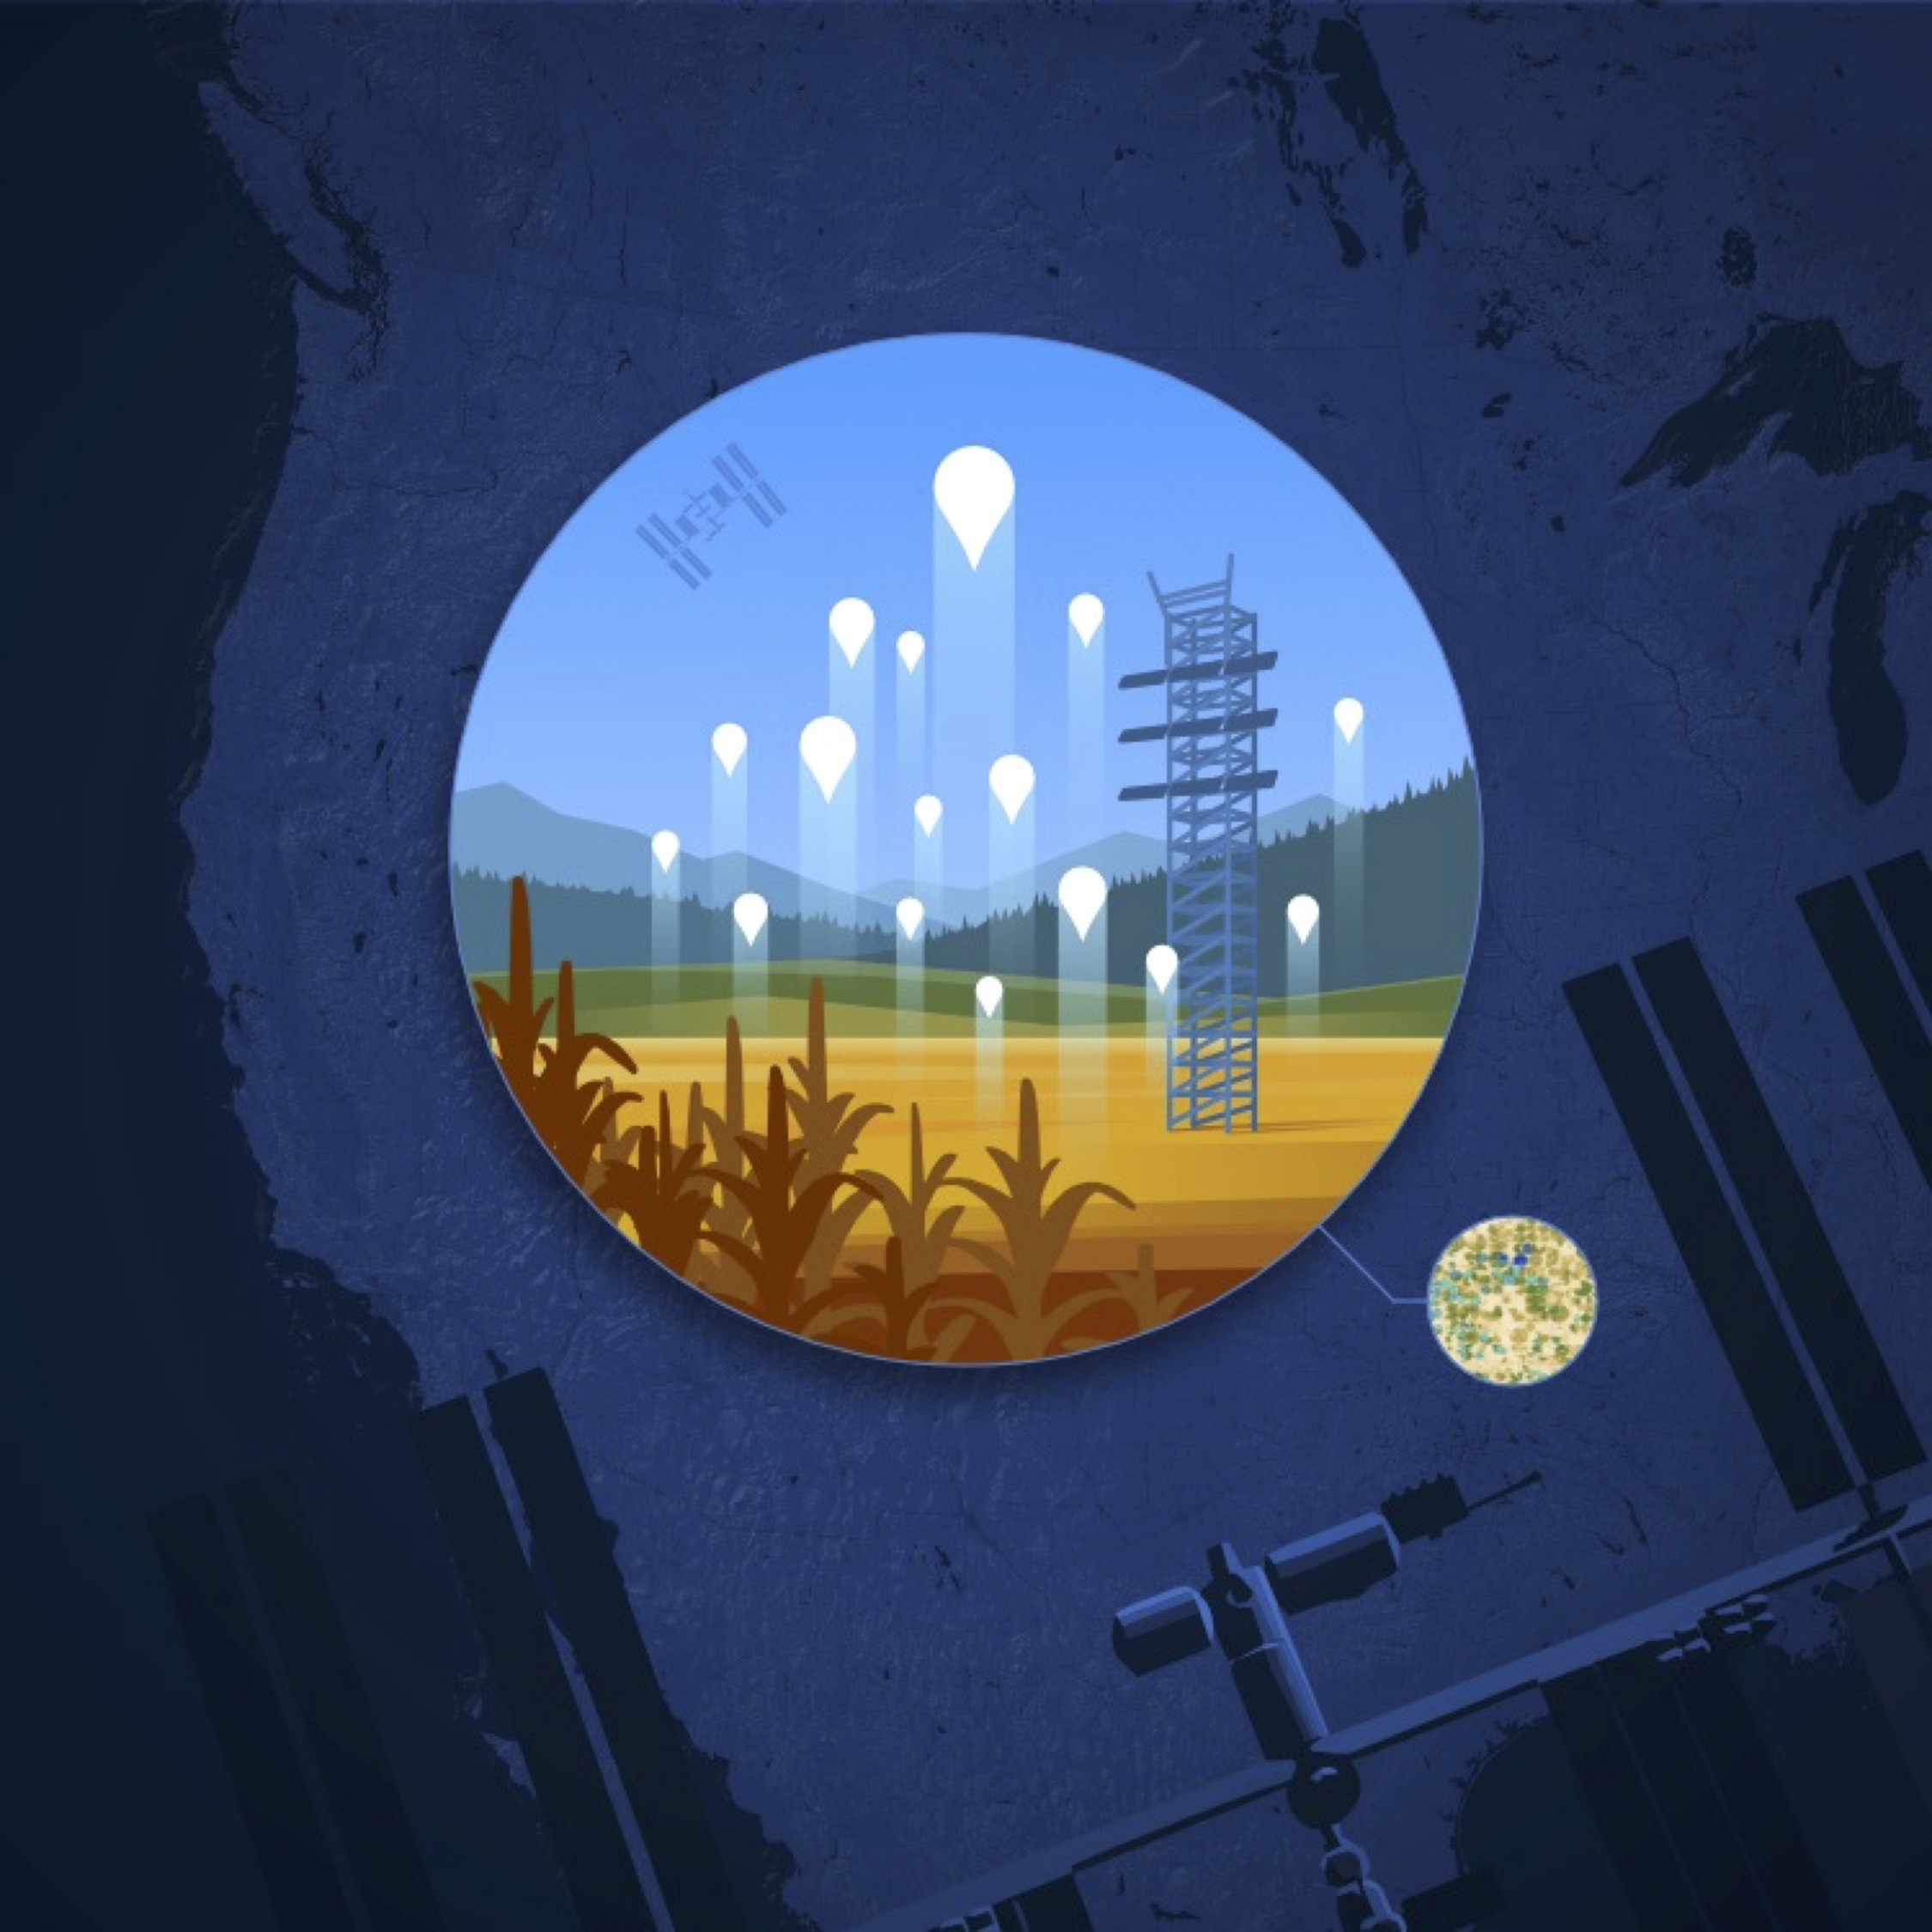
\includegraphics[scale=.03]{ECOSTRESS-BASE.jpg}};\end{tikzpicture}}
%%%%%%%%%%%%%%%%%%%%%%%%%%%%%%%%%%

\centerline{
\includegraphics[width=.65\textwidth]{QgisLogo.png}}

\section{Getting To Know QGIS}

First, you are going to familiarize yourself with QGIS, the software you downloaded in the previous tutorial:

On Windows, open QGIS Desktop from the start menu or desktop icon. 

On Mac, open QGIS by selecting it in Launchpad or use Go $\rightarrow$ Applications and double-click on QGIS.

Your screen will likely resemble something like this:

\centerline{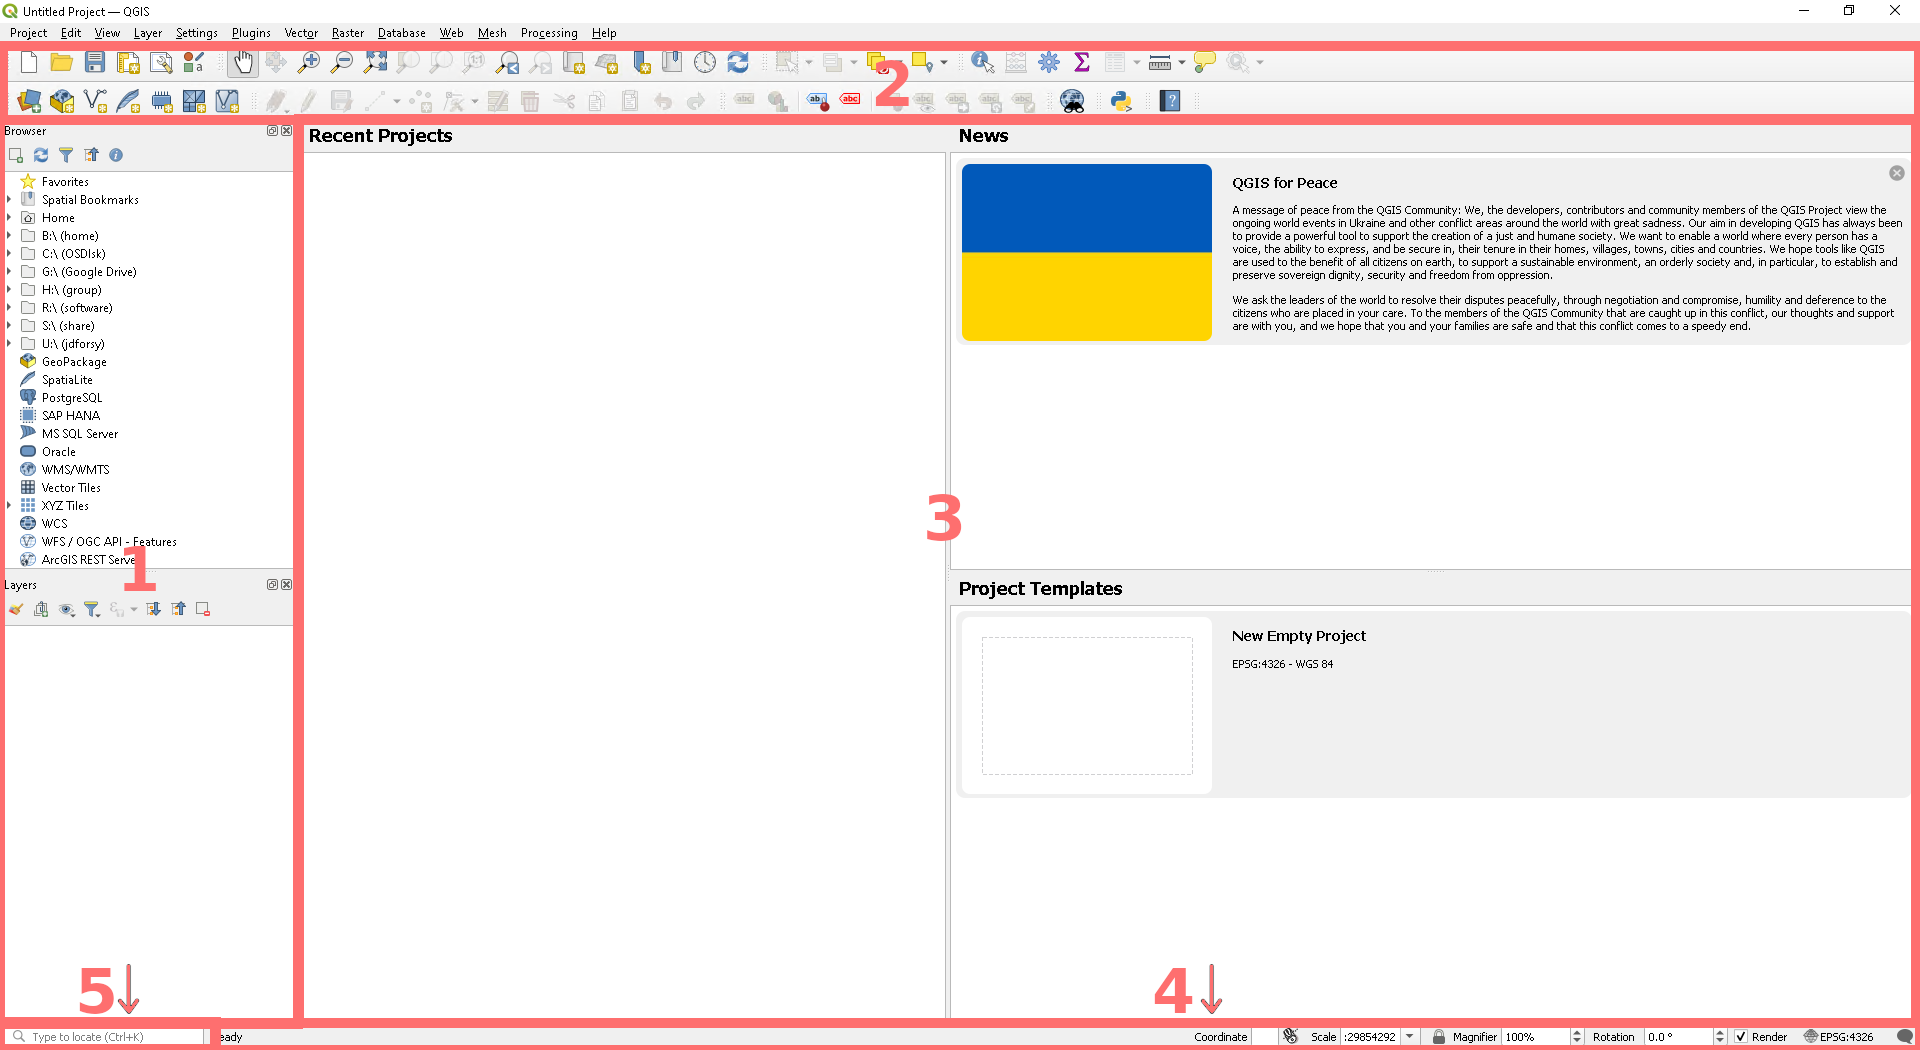
\includegraphics[width=\textwidth]{QGISscreen.png}}

\begin{enumerate}
	\item \textbf{Browser Panel \& Layers List}
	\begin{itemize}
		\item The browser panel lets you easily navigate files and databases. We will use it to import map layers and satellite data.
		\item In the layers list, you will see all the map layers we have imported for the given project we are working on. Layer examples include a base map (e.g., a Google map), satellite \href{https://en.wikipedia.org/wiki/Raster_graphics}{raster} data (e.g., pixels of temperature data from ECOSTRESS), and \href{https://en.wikipedia.org/wiki/Vector_graphics}{vector} data (e.g., points, lines, or shapes indicating points of interest, roads or buildings).
	\end{itemize}
	\item \textbf{Toolbars}
	\begin{itemize}
		\item The common tools can be found in the toolbars. For example, the *Project* toolbar allows you to save, load, print, and start a new project.
	\end{itemize}
	\item \textbf{Main Work Area / Map Canvas}
	\begin{itemize}
		\item The main work area is where the map itself is displayed. In the map canvas, you can interact with the visible layers: zoom in/out, move the map, select features, and complete many other operations.
	\end{itemize}
	\item \textbf{Status Bar}
	\begin{itemize}
		\item The status bar shows you information about the current map. Also allows you to adjust the map scale, the map rotation, and see the mouse cursor's coordinates on the map.
	\end{itemize}
	\item \textbf{Locator Bar}
	\begin{itemize}
		\item The locator bar allows you to quickly access almost all of the objects and functions of QGIS (e.g., layers, layer features, algorithms, spatial bookmarks, etc.) by typing in the search bar.
	\end{itemize}
\end{enumerate}

\section{Try It Out! Create Your First Map...}

\subsection{Add a Basemap Layer}

\centerline{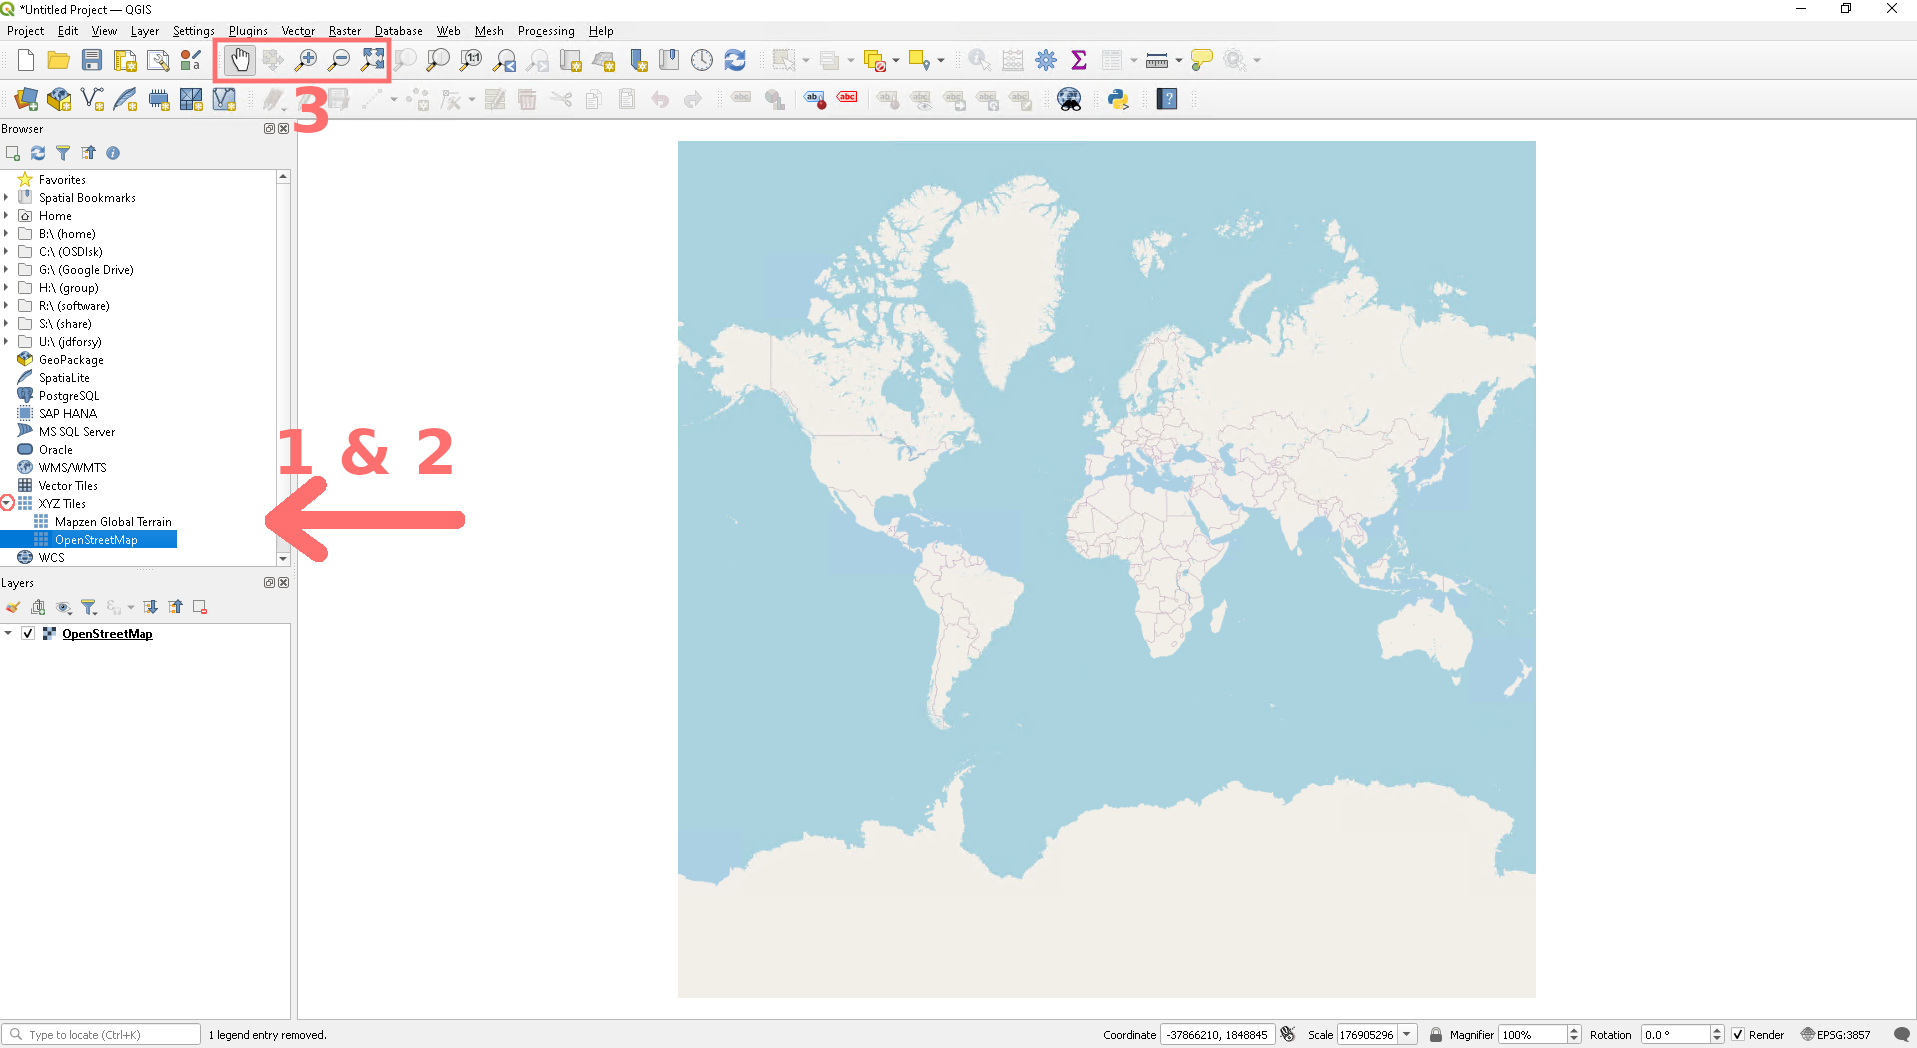
\includegraphics[width=\textwidth]{QGISbasemap.png}}

1. In the browser window, expand your options by clicking on the small arrow next to \textit{XYZ Tiles}.

2. Double-click on \textit{Open Street Map} to load in a basic open-source map. You will notice that we just added a layer to the layer window below.

3. You can zoom in and out with the magnifying glass icons in the toolbar. The little hand icon is the pan map function, which allows you to move the map around when you are zoomed in. Try finding your home or a favorite place in the world. To reset to the default view, you can use the icon of the magnifying glass with the arrows in all directions. 

\subsection{Add in an Interesting Layer via Shapefiles}

\href{https://en.wikipedia.org/wiki/Shapefile}{Shapefiles} are a common geospatial file type that stores locations, points, lines, and shapes.

1. Download this zipped folder from our website to your local computer:  \href{https://jeremydforsythe.github.io/icecream-tutorials/Tutorial2_MakingBasicMapsInQGIS/Time_Zones.zip}{US Timezones}. Make sure you save it to a dedicated project folder.

\centerline{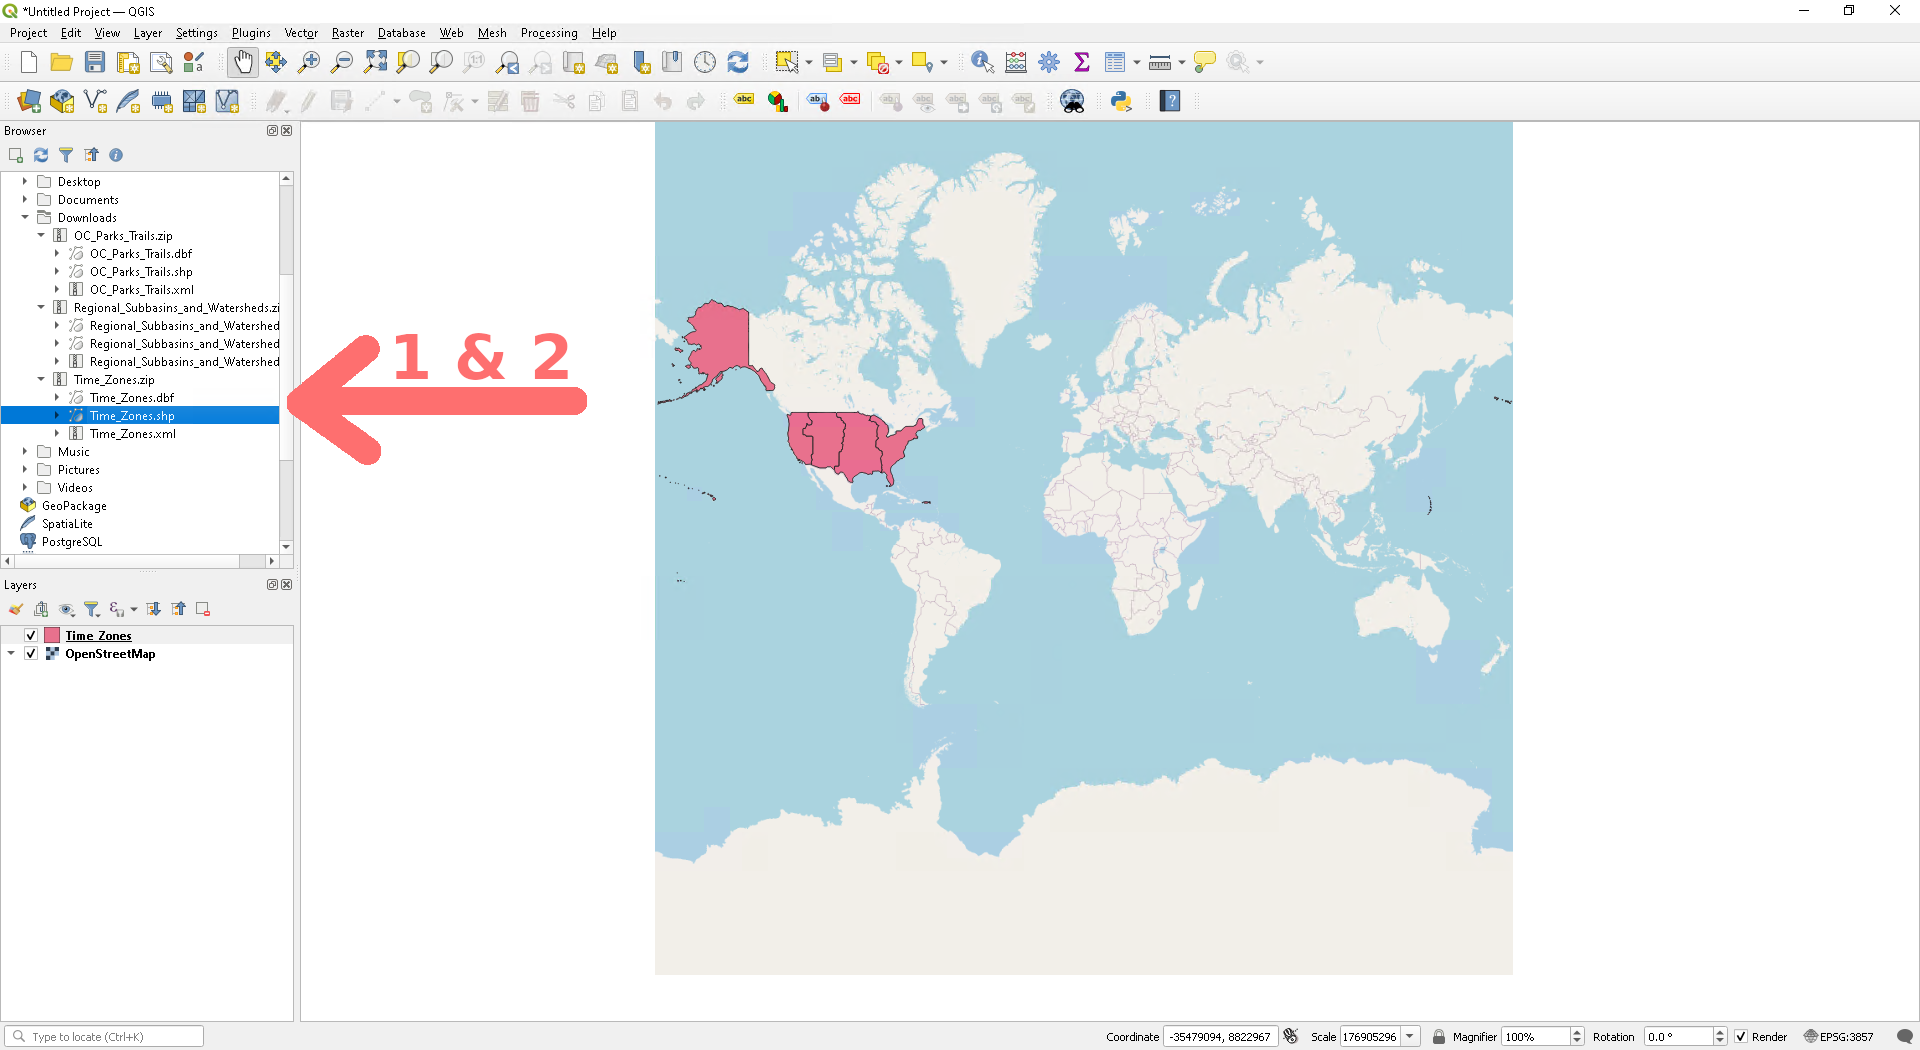
\includegraphics[width=\textwidth]{TimeZones.png}}

2. After you have downloaded the file, use the browser window to locate \textit{Time\textunderscore Zones.zip} in the folder in which you saved it. Use the little arrow to expand the zip file and double-click on the \textit{Time\textunderscore Zones.shp} shapefile. Similar to adding a base map, we have now added a new layer to our map.

\centerline{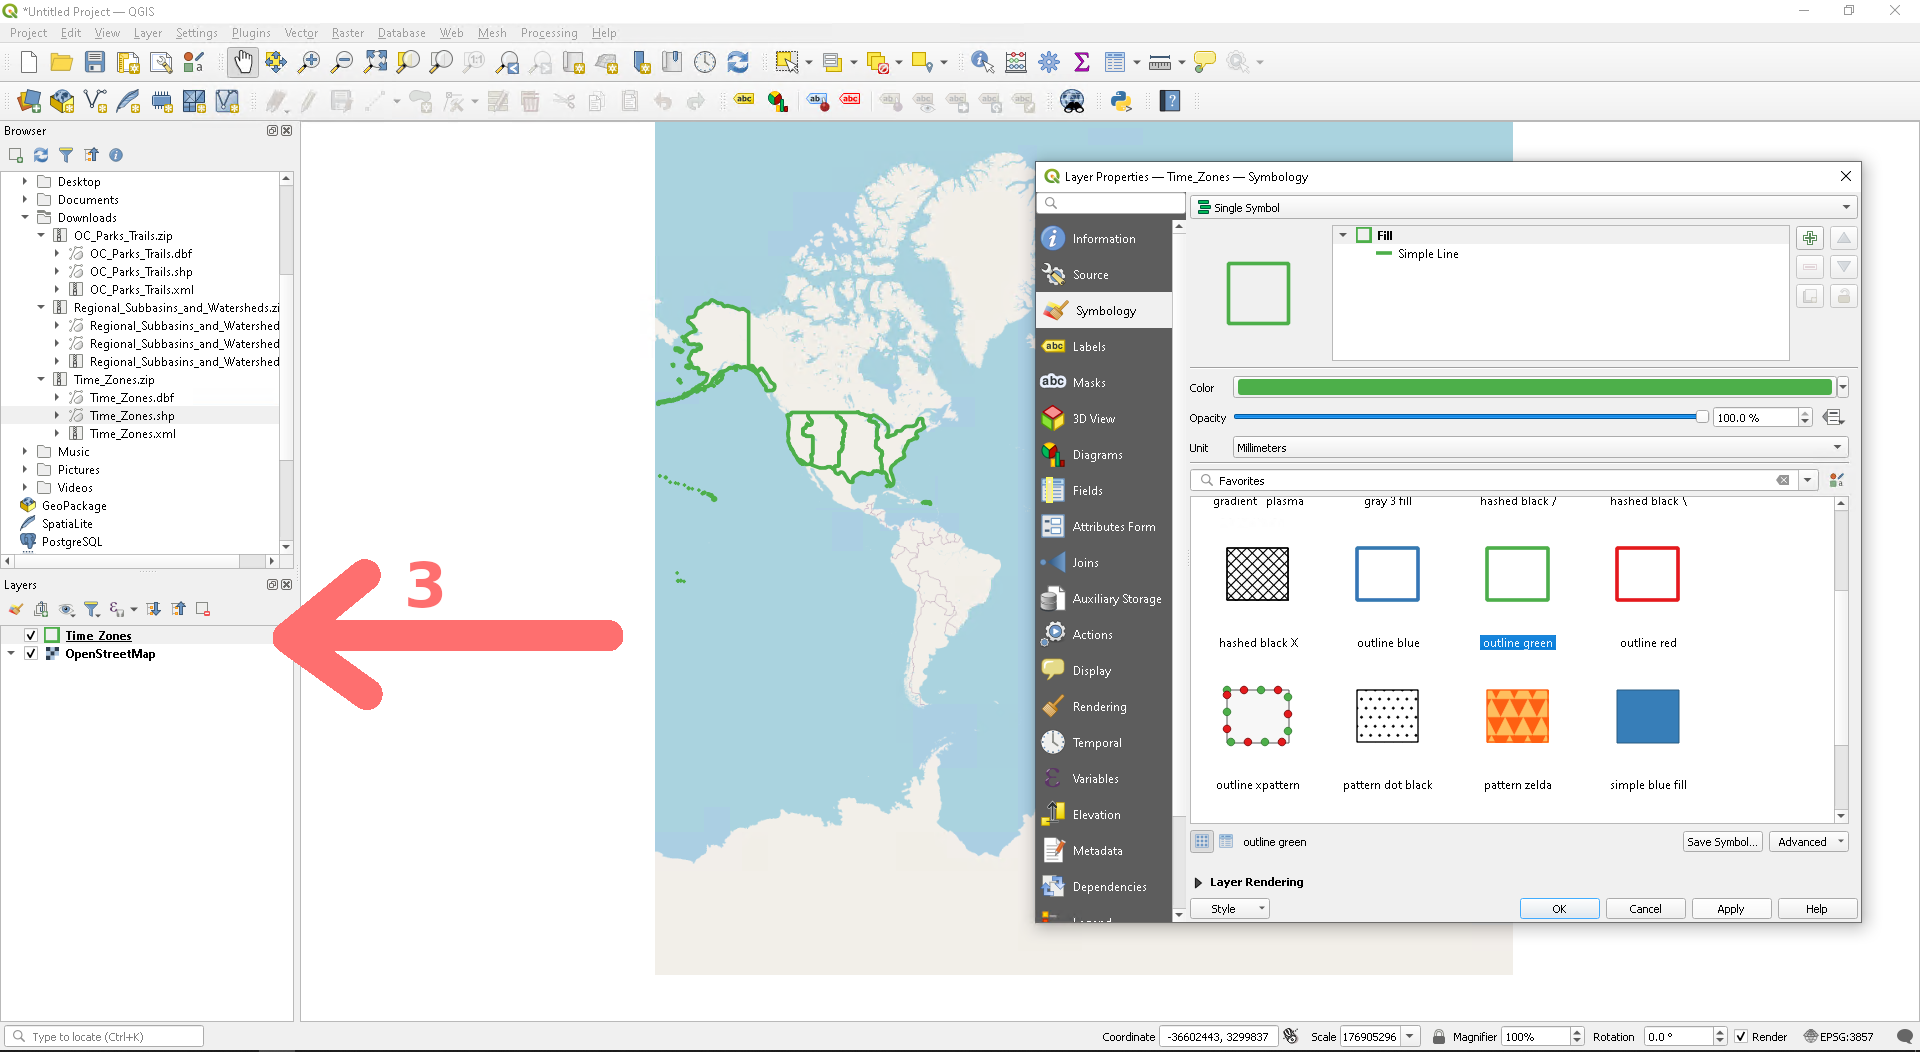
\includegraphics[width=\textwidth]{TimeZoneSymbol.png}}

3. This looks a little clunky, so let's make it more readable and useful. Right click on Windows/Linux, or control click on Mac, to open up the properties window. Navigate to the symbology window and select green outline. Click \textit{Apply} and \textit{OK}.  Then zoom and pan the map to center on North America, given that these are only US Timezones.

\centerline{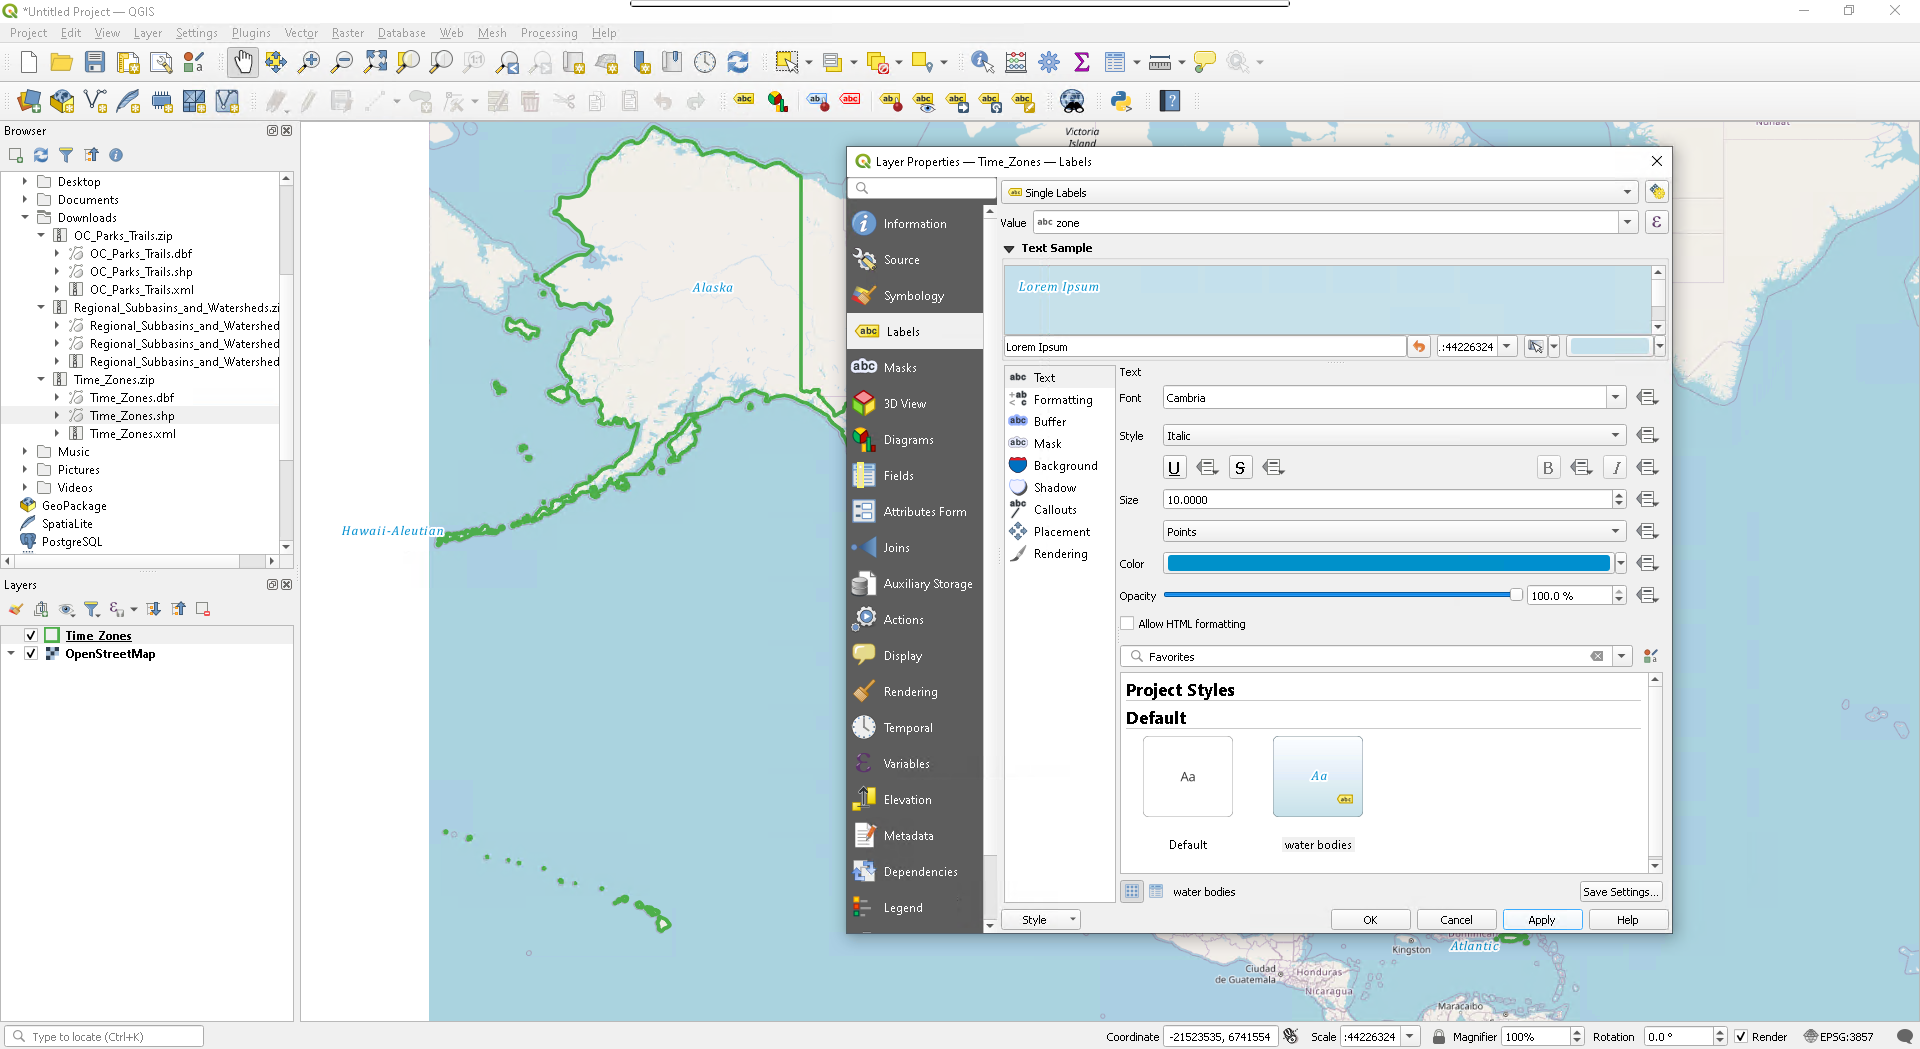
\includegraphics[width=\textwidth]{TimeZoneLabels.png}}

4. Next let's add labels. Re-open the properties window for Time Zones (i.e., right click) and navigate to the \textit{Labels} window. From the dropdown menu at the top select \textit{Single Labels}. Play around with the options to adjust the colors to your preferences, or maybe use one of the included styles (e.g., \textit{water bodies}). Click \textit{Apply} and \textit{OK}. 

\subsection{Exporting \& Sharing Your Map}

\centerline{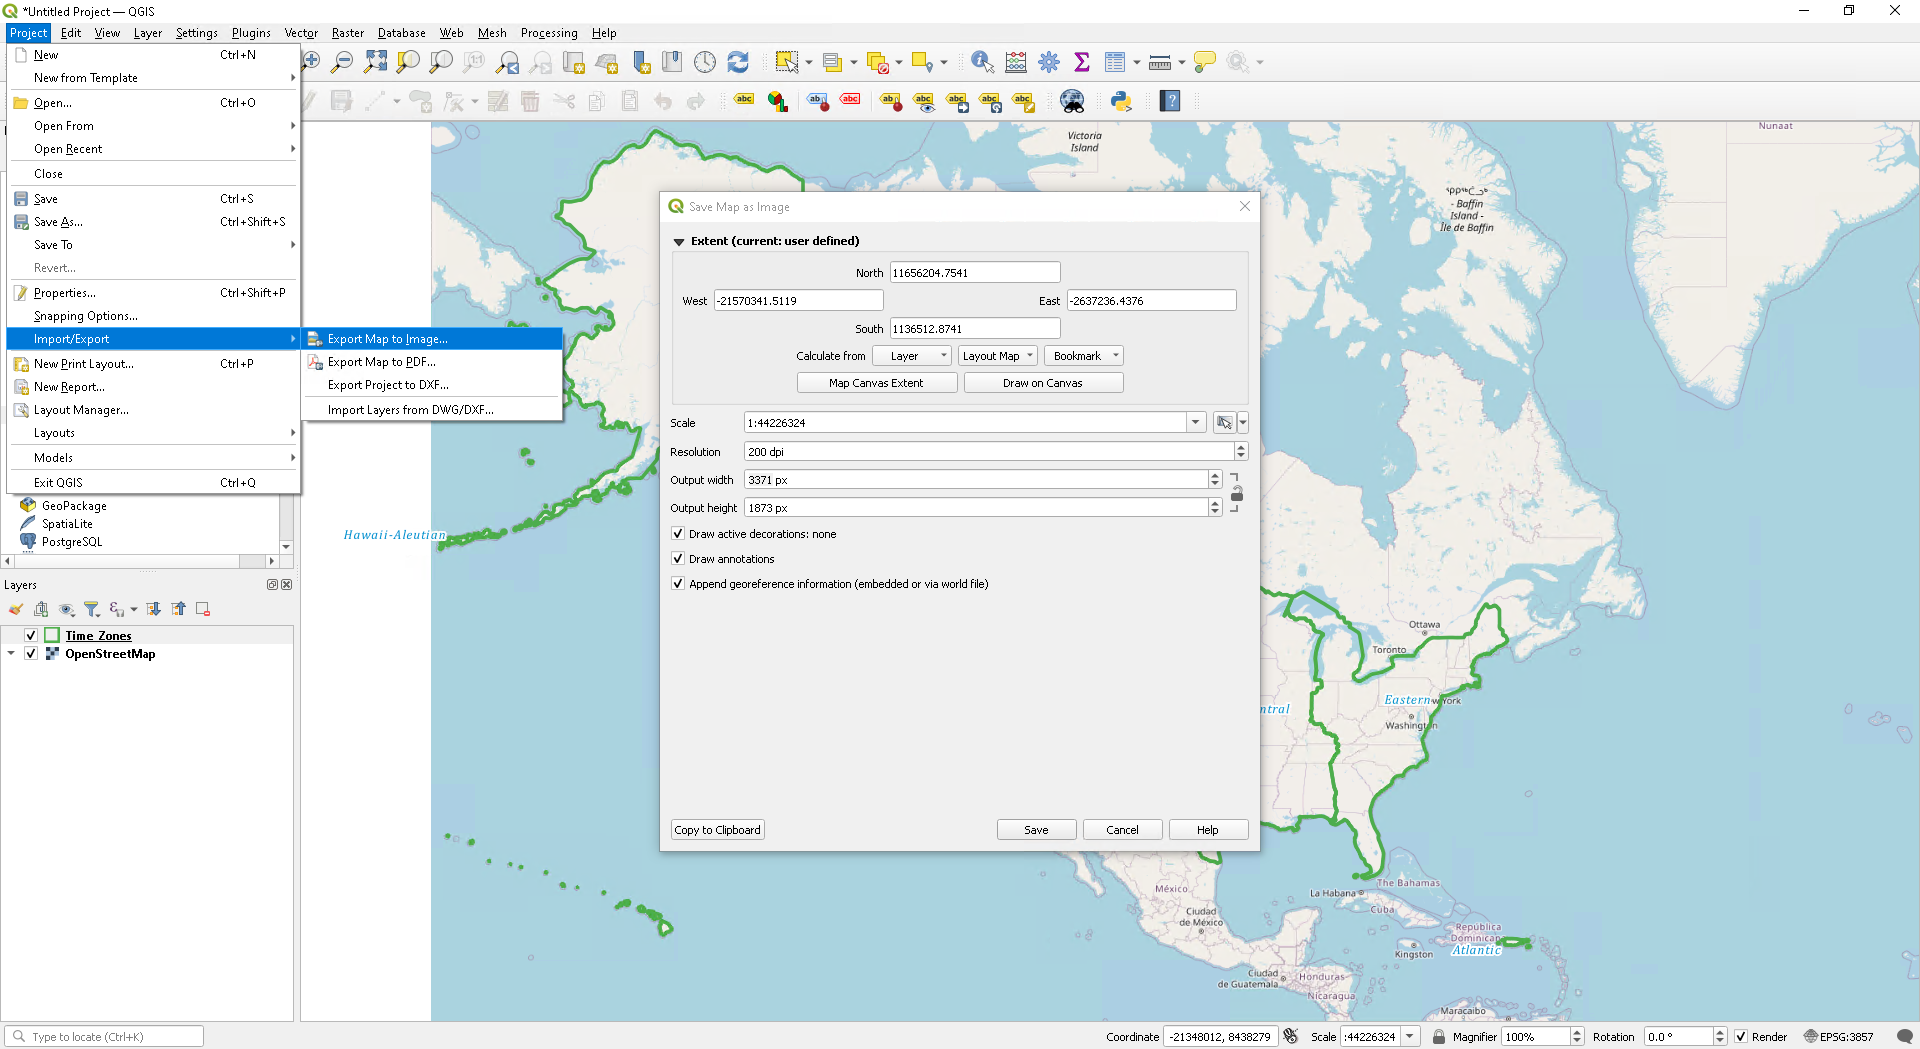
\includegraphics[width=\textwidth]{Export.png}}

5. Lastly, we want to save your map so you can marvel at your work anytime you'd like and share it with friends at parties. From the \textit{Project} menu, navigate to \textit{Import/Export} and select \textit{Export Map To Image}. By default, it will use the \href{https://en.wikipedia.org/wiki/Map_extent}{extent} that you have in the viewer. I recommend increasing the resolution to 200 DPI. You will submit this map later, so save it somewhere to your dedicated project folder. High-five! You have made a map. 


%%%%%%%%%%%%%%%%%%%%%%%%%%%%%%%%%%%%%%%%%%%%%%%%%%%%%%%%%%%%%%%%%%%%%%%%%%%%%%%%%%% End of Document
%\vfill

\hrule

\vspace{1em}

\small \textbf{Recommended Citation:} Forsythe, J.D., G.R. Goldsmith, and J.B. Fisher. 2023. Observing Earth from Above Tutorials. Chapman University. \url{https://jeremydforsythe.github.io/icecream-tutorials/}

\vspace{1em}

This work is supported by funding from NASA ECOSTRESS Mission Grant \#80NSSC23K0309 (I.C.E. C.R.E.A.M.: Integrating Communication of ECOSTRESS Into Community Research, Education, Applications, and Media) and is openly licensed via \href{https://creativecommons.org/licenses/by-nc/4.0/}{CC BY-NC}.

\end{document}
